

\usepackage{xcolor}


%%novalidate

\usepackage{tikz}
\usepackage{calc}
\usepackage{booktabs}
\usepackage{tcolorbox}
\usepackage{pgfkeys}
\tcbuselibrary{listings,breakable,skins}
\usetikzlibrary{shadings}
%\usepackage{hyperref}

% colors
\definecolor{color1}{HTML}{0267c1}
%\definecolor{color1}{HTML}{8C260F}
\definecolor{color2}{HTML}{591f0a}


% fonts
%\usepackage[english, brazilian]{babel}
\usepackage{fontspec}
\defaultfontfeatures{Mapping=tex-text}


%\setmainfont
%[BoldFont=Lato/Lato-Bold.ttf,
%ItalicFont=Lato/Lato-Italic.ttf,
%BoldItalicFont=Lato/Lato-BoldItalic.ttf]
%{Lato/Lato-Regular.ttf}
%\newfontfamily\headingfont[ItalicFont=Lato/Lato-BlackItalic.ttf,ExternalFont={Lato/Lato-Black.ttf}]{Lato-Black.ttf}
\IfFontExistsTF{Arial Black}
  {\newfontfamily\headingfont{Arial Black}}
  {\newfontfamily\headingfont[Path=fonts/]{Lato-Black.ttf}}

%%%

\usepackage{geometry}
\geometry{a4paper,
hmargin=30mm,vmargin=30mm,
head=0ex,foot=5ex}

\linespread{1.3}

\usepackage[hang]{caption}
\DeclareCaptionFormat{upper}{#1#2\uppercase{#3}\par}
\captionsetup{labelfont={bf,color=color2},textfont={normalsize,color=color2},format = upper,figurename=FIGURA,tablename=TABELA}
\AtBeginDocument{\hypersetup{pdflang={pt-BR}}}
\AddToHook{begindocument/end}{%
  \renewcommand*\listfigurename{Lista de figuras}%
  \renewcommand*\listtablename{Lista de tabelas}%
}

\let\paragraph\oldparagraph
\let\subparagraph\oldsubparagraph

%%% fancy sections
\usepackage{titlesec}
%\titleformat{\chapter}{\headingfont\LARGE\bfseries\scshape\color{color1}}{\thechapter}{1em}{}[\titlerule]
\titleformat{\section}{\color{color1}\headingfont\Large\bfseries\uppercase}{\thesection}{1em}{}[\titlerule]
\titleformat{\subsection}{\color{color2}\headingfont\large\bfseries\uppercase}{\thesubsection}{1em}{}
\titleformat{\subsubsection}{\color{color1}\headingfont\bfseries\uppercase}{\thesubsubsection}{1em}{}
%%%


% head and foot
\usepackage{fancyhdr}
\pagestyle{fancy}
\lhead{}
\chead{}
\makeatletter
\rhead{\color{color2}\@date}
\makeatother
\newlength{\myheight}
\lfoot{
\settoheight{\myheight}{\thepage}
\raisebox{-2ex-0.5\myheight}{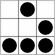
\includegraphics[height=4ex]{logo}}
}
\cfoot{\color{color2}EPS2361 · Análise de Dados}
\rfoot{\color{color2}\thepage}
\renewcommand\headrulewidth{0pt}
\renewcommand\footrulewidth{0pt}
%%%

%%% picture on cover page
\usepackage{eso-pic}
\newcommand\BackgroundPic{%
\put(0,0){%
\parbox[b][\paperheight]{\paperwidth}{%
\vfill
\centering

\includegraphics[width=\paperwidth,height=\paperheight,%
keepaspectratio]{cover}%
\vfill
}}}
%%%


%%%
% custom titlepage
\makeatletter
\renewcommand{\maketitle}{
\thispagestyle{empty}
\AddToShipoutPicture*{\BackgroundPic}
\AddToShipoutPictureFG*{\AtPageLowerLeft{%
  \put(\LenToUnit{.342\paperwidth},\LenToUnit{.156\paperheight}){%
    \parbox[t]{.49\paperwidth}{\raggedright\color{white}\fontsize{11}{13}\selectfont\@title}}%
  \put(\LenToUnit{.342\paperwidth},\LenToUnit{.122\paperheight}){%
    \parbox[t]{.49\paperwidth}{\raggedright\color{white}\fontsize{10}{12}\selectfont\@author}}%
}}
\null
\clearpage
}
\makeatother
%%%

%%% fancy boxes
\usepackage{tcolorbox}
\usepackage{wrapfig}
\def\fullboxbegin{
\bigskip
\begin{tcolorbox}[colback=color1,colframe=color1,coltext=white,arc=0mm,boxrule=0pt]
}
\def\fullboxend{\end{tcolorbox}\medskip}
%
\def\leftboxbegin{
\begin{wrapfigure}{l}{0.5\textwidth}
\begin{tcolorbox}[colback=color1,colframe=color1,coltext=white,arc=0mm,boxrule=0pt]
}
\def\leftboxend{
\end{tcolorbox}
\end{wrapfigure}
}
%
\def\rightboxbegin{
\begin{wrapfigure}{r}{0.5\textwidth}
\begin{tcolorbox}[colback=color1,colframe=color1,coltext=white,arc=0mm,boxrule=0pt]
}
\def\rightboxend{
\end{tcolorbox}
\end{wrapfigure}
}
%
\newcounter{frames}
\def\frameboxbegin#1{
\bigskip
\refstepcounter{frames}
\begin{tcolorbox}[colback=white,colframe=color1,arc=0mm,title={\MakeUppercase{\textbf{Frame \arabic{frames}}: #1}}]
}
\def\frameboxend{
\end{tcolorbox}
}
%%%
